\documentclass[
  11pt,
  letterpaper,
   addpoints,
   answers
  ]{exam}
\usepackage{../exercise-preamble}
\usepackage{float}
\usepackage{subcaption}
\usepackage{circuitikz}  % tal como ya lo tienes
\ctikzset{current/american}


\begin{document}

\noindent
\begin{minipage}{0.47\textwidth}

\includegraphics[width=\textwidth]{../fcfm_die}
\end{minipage}
\begin{minipage}{0.53\textwidth}
\begin{center} 
\large\textbf{Circuitos Eléctricos Analógicos} (EL3202-1) \\
\large\textbf{Clase auxiliar 4} \\
\normalsize Prof.~ Patricio Mendoza.\\
\normalsize Prof.~Aux.~Renato Planas ~Erik Sáez
\end{center}
\end{minipage}

\vspace{0.5cm}
\noindent
\vspace{.85cm}

\begin{questions}
%----------------------------
\question
Para el circuito de la Figura~\ref{fig:1}, si utiliza la expresión exacta $I(v_D)$ del diodo, plantee la ecuación que se debe satisfacer. Plantee un modelo de aproximación para el diodo que permita resolver los voltajes y corrientes en el circuito. Sea explícito en los modelos y supuestos utilizados.
\begin{equation}
  i_D = I_s \left( e^{v_D/(\eta V_T)} - 1 \right)
\end{equation}

\begin{figure}[H]
    \centering
    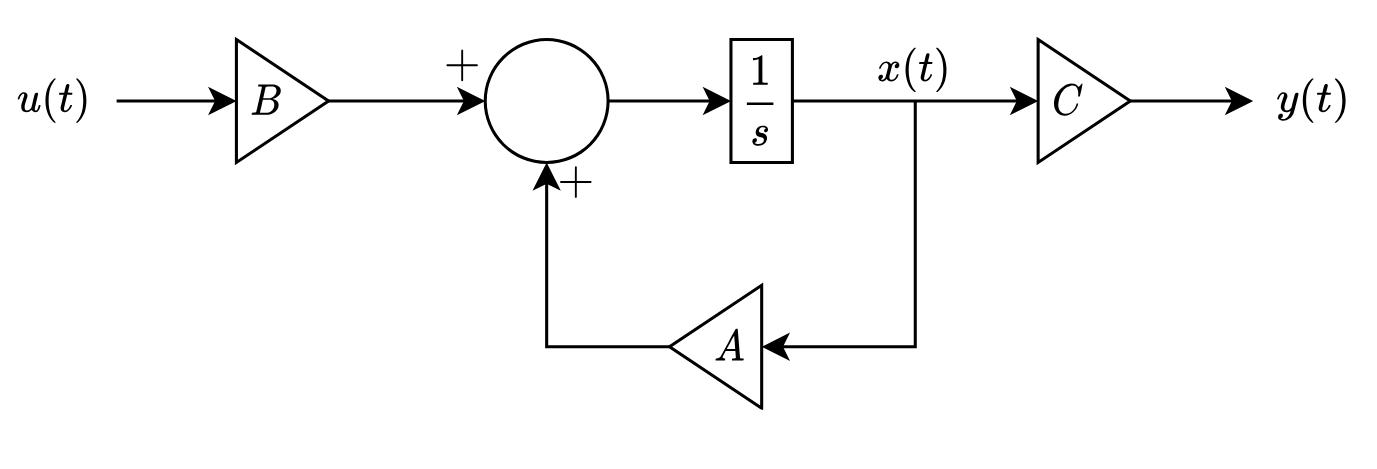
\includegraphics[width=0.8\textwidth]{Auxiliar_4_1}
    \caption{Circuito con diodo.}
    \label{fig:1}
\end{figure}
%----------------------------
\newpage
\begin{solution}
Un diodo es un dispositivo semiconductor que permite el paso de corriente en una sola dirección y presenta caracteristicas no lineales. La curva $v$ -- $i$ se puede visualizar en la figura \ref{fig:th_norton_1}:
\begin{figure}[H]
    \centering
    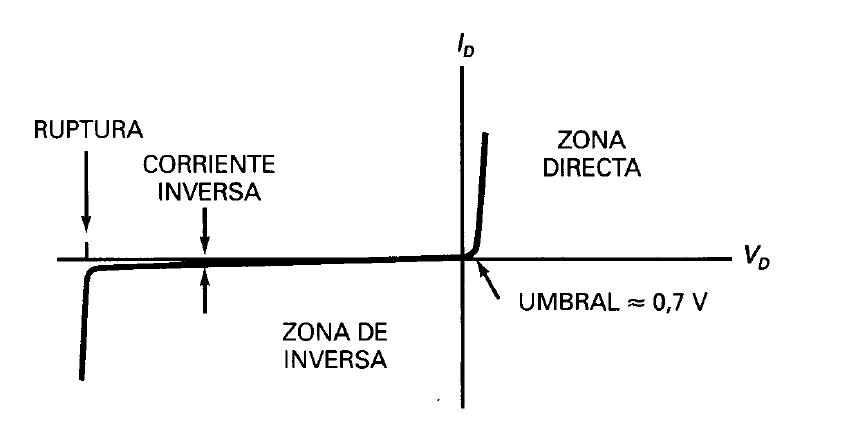
\includegraphics[width=0.8\textwidth]{Auxiliar_4_27}
  \caption{Característica $v$--$i$ del diodo. Se observa la zona directa, donde para $v_D > 0{,}7\,$V (diodo de silicio) la corriente $i_D$ crece rápidamente y el diodo conduce; el umbral de conducción cerca de $0{,}7\,$V; la zona inversa, donde para $v_D < 0$ la corriente es muy pequeña (corriente inversa de saturación); y la zona de ruptura, donde si el voltaje inverso supera un valor crítico, la corriente inversa aumenta bruscamente. Estas regiones son fundamentales para el análisis de circuitos con diodos.}
    \label{fig:th_norton_1}
\end{figure}
Ademas tenemos que la curva $v$ -- $i$ depende fuertemente de la temperatura a la cual estemos operando. Por otro lado la curva que modela el comportamiento del diodo viene dado por la ecuación de Shockley,
\begin{align}
    i_D &= I_s\left(e^{\frac{v_D}{\eta V_T}} - 1\right) 
\end{align}
Donde cada termino corresponde a:
\begin{itemize}
    \item $i_D$: corriente a través del diodo.
    \item $I_s$: corriente de saturación del diodo.
    \item $v_D$: voltaje a través del diodo.
    \item $\eta$: factor de idealidad del diodo el cual toma en cuenta las propiedades del material y para un caso ideal $\eta = 1$.
    \item $V_T$: voltaje térmico, que depende de la temperatura.
\end{itemize}
Ademas existe el denominado punto de operacion, el cual describe el estado en el cual se encuentra el diodo, y este depende de la corriente y voltaje que lo atraviesan. El punto de operación se determina por la intersección entre la característica $v$--$i$ del diodo y la recta de carga del circuito externo al diodo. La recta de carga representa la relación entre voltaje y corriente impuesta por el circuito externo al diodo. La intersección con la característica $v$–$i$ del diodo determina el punto de operación.
Volviendo sobre el problema se tiene enunciado, debemos utilizar la expresión exacta del diodo, considerando temperatura ambiente. Por lo tanto, tenemos que $V_{T}=25\,\mathrm{mV}$. La ecuación exacta que describe el comportamiento del diodo es:
Por enunciado, debemos utilizar la expresión exacta del diodo, considerando temperatura ambiente. Por lo tanto, tenemos que $V_{T}=25\,\mathrm{mV}$. La ecuación exacta que describe el comportamiento del diodo es:
\begin{align}
    i_D &= I_s\left(e^{\frac{v_D}{\eta V_T}} - 1\right) \label{eq:shockley}\\
    &= 10^{-5}mA\left(e^{\frac{v_D}{2 \cdot 25[mV]}} - 1\right)\\
    &=10^{-5}mA(e^{20v_{D}}-1)
\end{align}
donde $I_s$ es la corriente de saturación y $\eta$ el factor de idealidad ($1 \leq \eta \leq 2$). En este ejercicio se considera $\eta = 2$ según el enunciado. Por la Ley de Corriente de Kirchhoff (LCK) en el nodo del diodo:
\begin{align}
    i_1 &= i_2 + i_3 \\
\frac{V_i - v_D}{R_1} &= \frac{v_D}{R_2} + I_s\left(e^{\frac{v_D}{\eta V_T}} - 1\right) \label{eq:kcl}
\end{align}
 
 Si suponemos que $v_D = 0{,}7\,\mathrm{V}$, el cual es un valor común para un diodo de silicio en conducción, tenemos:
  \begin{align*}
    i_1 &= \frac{V_i - v_D}{R_1} = \frac{12 - 0{,}7}{10\,000}\ \mathrm{A} = 1{,}13\ \mathrm{mA} \\
    i_2 &= \frac{v_D}{R_2} = \frac{0{,}7}{10\,000}\ \mathrm{A} = 70\ \mu\mathrm{A} \\
    i_3 &= i_1 - i_2 = 1{,}06\ \mathrm{mA}
  \end{align*}
  Si en vez de $v_D = 0{,}7\,\mathrm{V}$ usamos $v_D = 0{,}6\,\mathrm{V}$:
  \begin{align*}
    i_1 &= \frac{12 - 0{,}6}{10\,000} = 1{,}14\ \mathrm{mA} \\
    i_2 &= \frac{0{,}6}{10\,000} = 60\ \mu\mathrm{A} \\
    i_3 &= i_1 - i_2 = 1{,}08\ \mathrm{mA}
  \end{align*}
Vemos que obtenemos valores bastante pequeños para la corriente del diodo, lo que puede parecer contradictorio, pero esto se debe al punto de operación en el que se encuentra el diodo. Ahora analizaremos dos situaciones límite para el diodo:
\begin{itemize}
    \item \textbf{Caso 1: Diodo en corte ($i_D = 0$)}. El diodo no conduce corriente y se comporta como un circuito abierto:
    \begin{figure}[H]
      \centering
      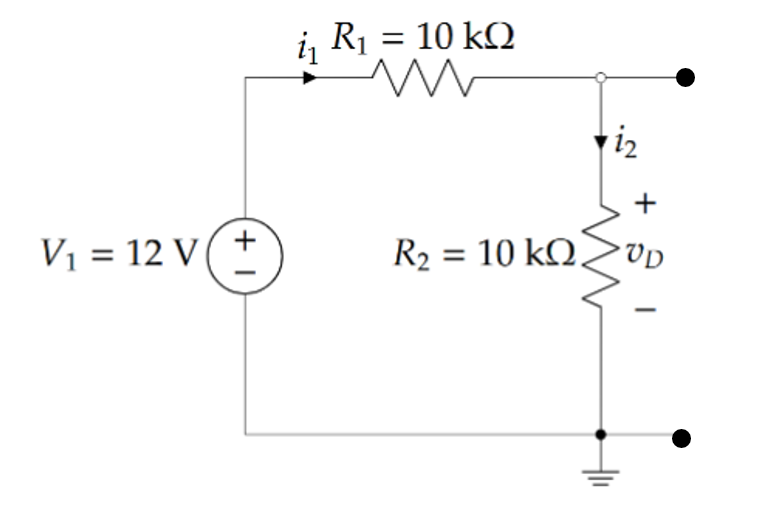
\includegraphics[width=0.4\textwidth]{Auxiliar_4_10}
      \caption{Circuito con diodo abierto.}
      \label{fig:th_norton_2}
    \end{figure}
  El voltaje en el diodo será:
    \begin{align*}
        12 &= (R_1 + R_2)i \\
        i &= \frac{12}{20\,000} = 0{,}6\ \mathrm{mA} \\
        v_D &= R_2 i = 10\,000 \times 0{,}6\ \mathrm{mA} = 6\ \mathrm{V}
    \end{align*}
    \item \textbf{Caso 2: Diodo en conducción (cortocircuito ideal)}. El diodo conduce y se comporta como un corto:
    \begin{figure}[H]
      \centering
      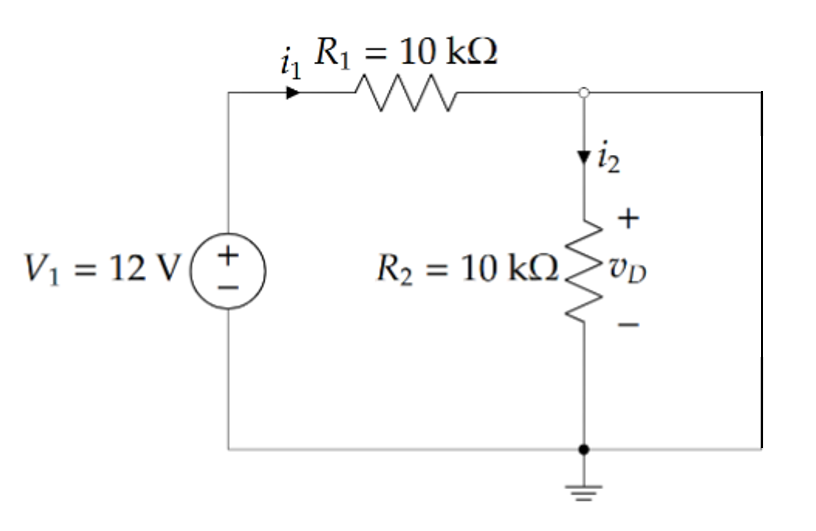
\includegraphics[width=0.4\textwidth]{Auxiliar_4_11}
      \caption{Circuito con diodo en corto circuito.}
      \label{fig:th_norton_3}
    \end{figure}
  En este caso, por la resistencia $R_2$ no circula corriente alguna:
    \begin{align*}
        12 &= R_1 i \\
        i &= \frac{12}{10\,000} = 1{,}2\ \mathrm{mA}
    \end{align*}
    Cuando $v_D = 0$, la corriente es $1{,}2\ \mathrm{mA}$.
\end{itemize}

La recta de carga representa la relación entre voltaje y corriente impuesta por el circuito externo al diodo. La intersección con la característica $v$–$i$ del diodo dada por \eqref{eq:shockley} determina el punto de operación. En este caso, el voltaje de intersección resulta menor que $0{,}6\,\mathrm{V}$ y, por la forma exponencial de \eqref{eq:shockley}, la corriente del diodo queda del orden de miliamperes. Para aumentar la corriente de operación, habría que modificar la recta de carga (por ejemplo, disminuyendo las resistencias o aumentando $V_i$).

\begin{figure}[H]
  \centering
  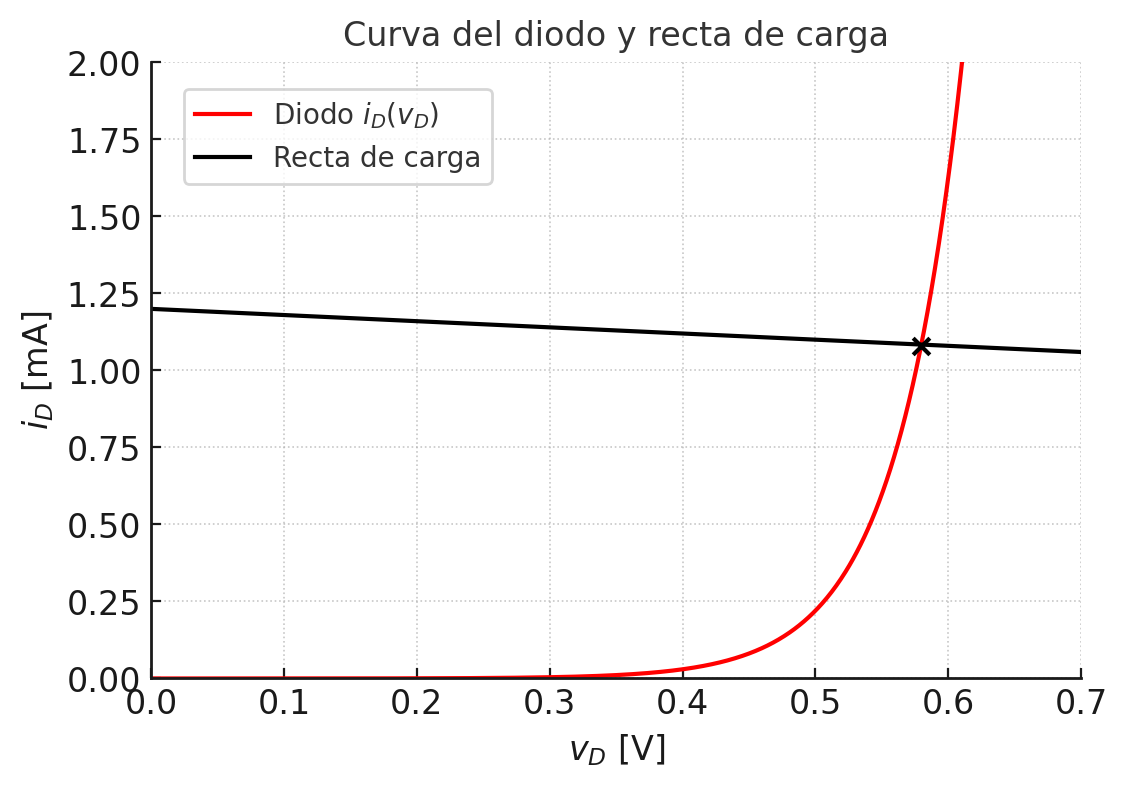
\includegraphics[width=0.6\textwidth]{Auxiliar_4_2}
  \caption{Intersección entre la característica $v$–$i$ del diodo y la recta de carga del equivalente de Thévenin.}
  \label{fig:th_norton_6}
\end{figure}


\end{solution}
\newpage
%----------------------------
    \question Un diodo Zener con característica $v$--$i$, como la mostrada en la Figura 5a), tiene un voltaje de Zener
    $V_{ZK}=3\ \mathrm{V}$. Determine la corriente $i_X$ en los dos circuitos mostrados en la figura \ref{fig:ex4c}. Sea explícito en los modelos y supuestos utilizados.  

% --- Figuras de los dos casos ---
\begin{figure}[H]
  \centering

  \begin{subfigure}[b]{0.48\textwidth}
    \centering
    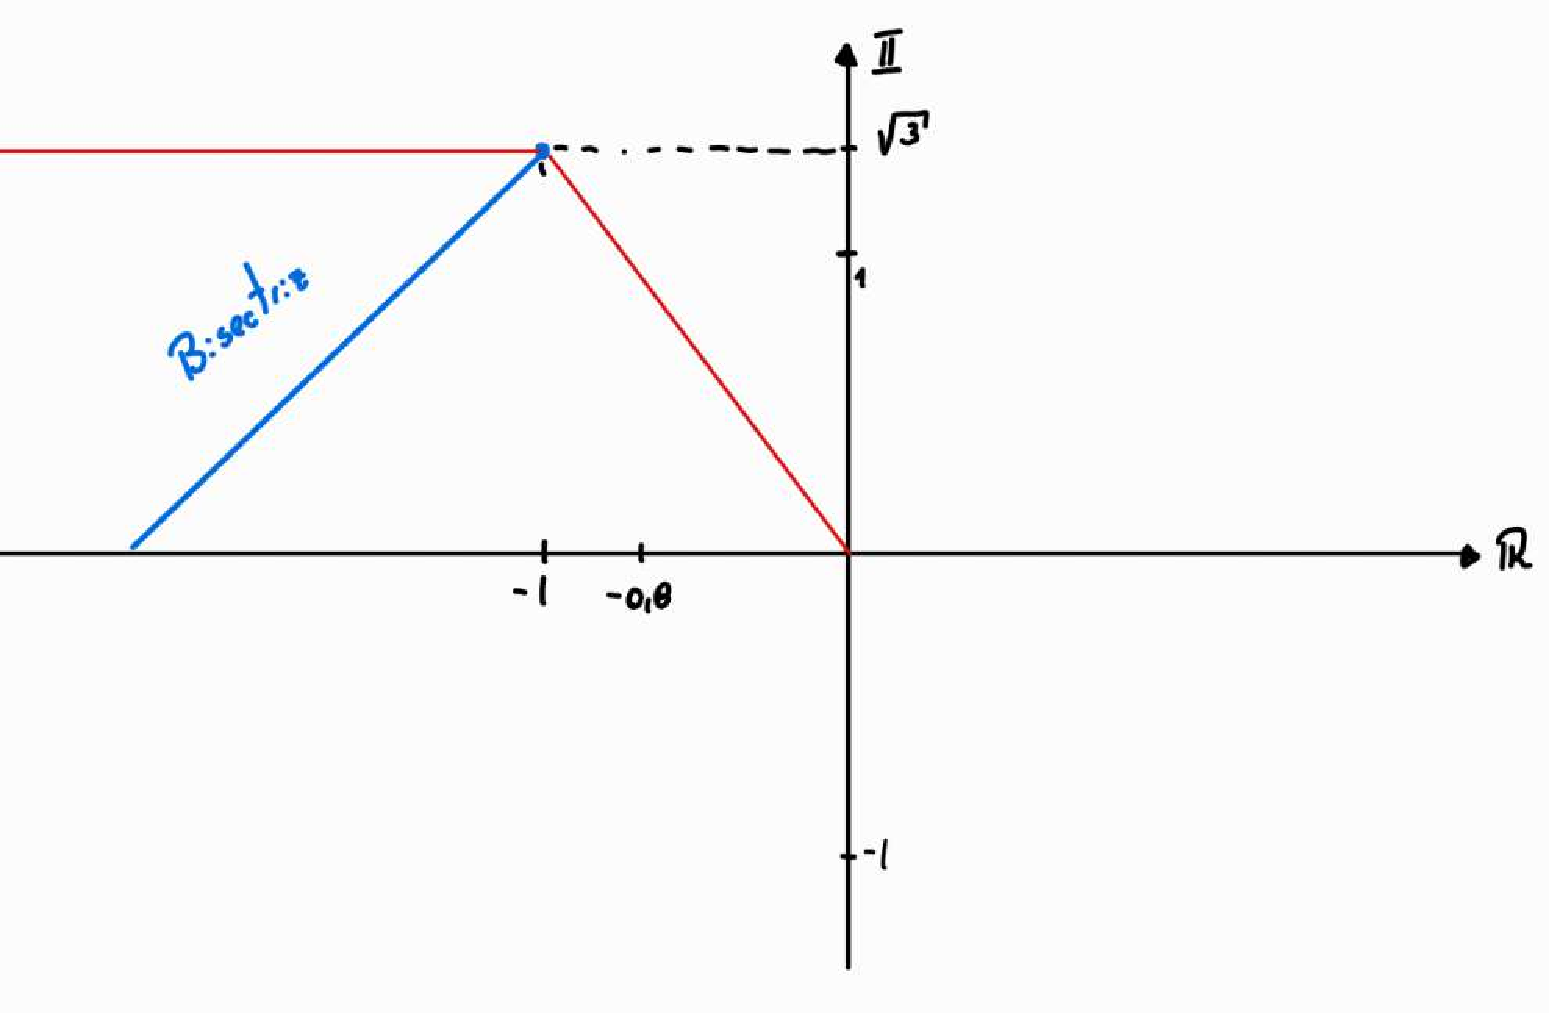
\includegraphics[width=1\linewidth]{Auxiliar_4_5}
    \caption{Curva de v-i del diodo Zener.}
    \label{fig:ex4a}
  \end{subfigure}\hfill
  \begin{subfigure}[b]{0.48\textwidth}
    \centering
    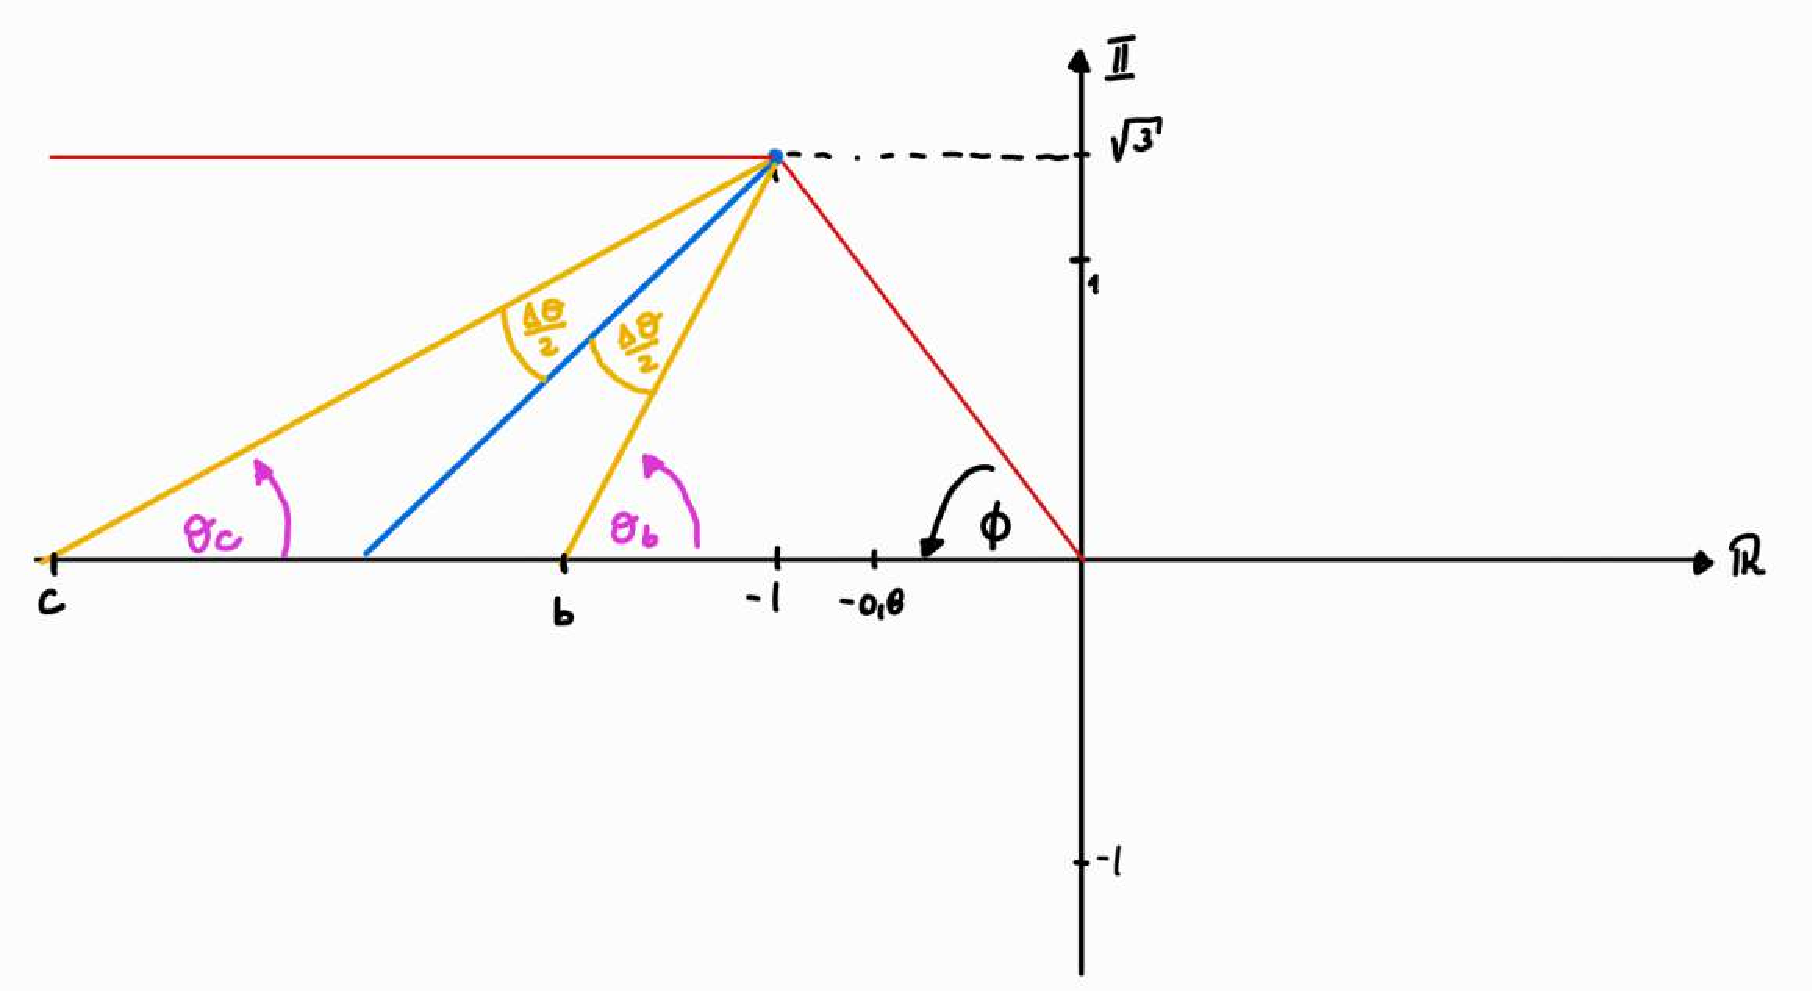
\includegraphics[width=0.5\linewidth]{Auxiliar_4_6}
    \caption{Esquema de un diodo Zener.}
    \label{fig:ex4b}
  \end{subfigure}

  \caption{ (a) Característica $v$--$i$ del diodo Zener, mostrando las regiones de polarización directa, inversa y de ruptura inversa, así como los valores típicos de voltaje y corriente. (b) Símbolo del diodo Zener, mostrando la dirección de la corriente $i_Z$ y el voltaje $v_Z$ en sus terminales.}
  \label{fig:ex4ab}
\end{figure}

% --- Hueco para la figura de detalle v-i ---
\begin{figure}[H]
  \centering  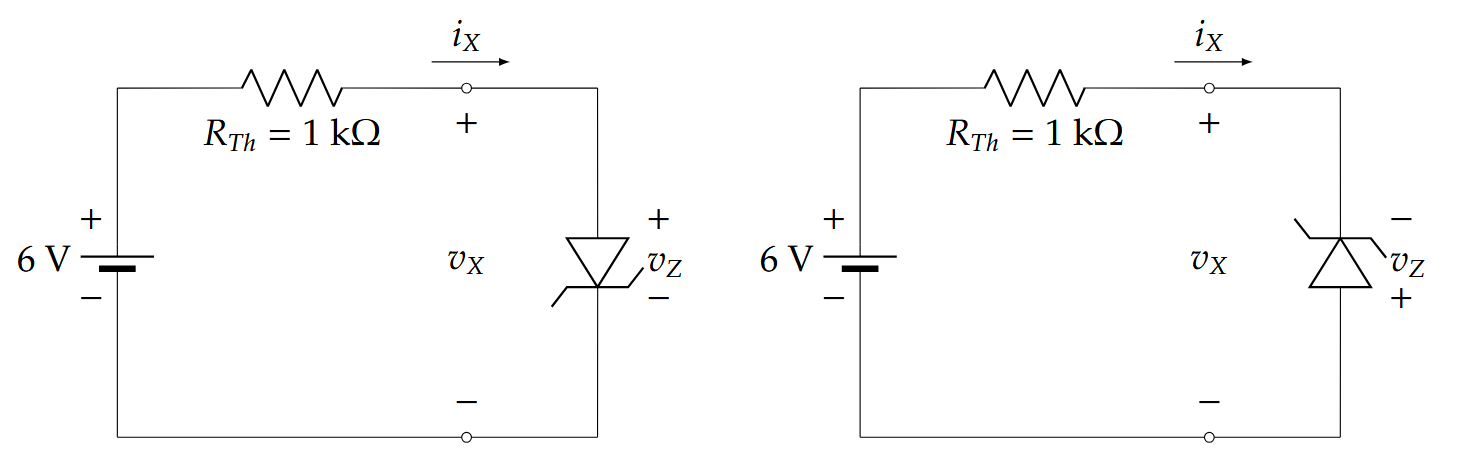
\includegraphics[width=0.8\textwidth]{Auxiliar_4_7}
  \caption{Detalle: (izquierda) símbolo del diodo Zener con convención de corriente $i_Z$ y polaridad de $v_Z$; (derecha) característica $v$--$i$ esquemática del diodo (ruptura inversa alrededor de $-V_{ZK}$).}
  \label{fig:ex4c}
\end{figure}

%----------------------------
\begin{solution}

Similar a lo anterior, tenemos que el primer paso en este problema es encontrar la recta de carga que describe a la fuente de voltaje y a la resistencia de Thévenin. Para esto notemos que cuando la corriente \(i_X\) es igual a cero, entonces no hay una caída de voltaje en la resistencia, por lo que el voltaje \(v_X\) es igual al voltaje de la fuente, es decir, \(6~\text{V}\). Si el voltaje \(v_X\) es cero, entonces el diodo actúa como un cortocircuito y tenemos que la corriente \(i_X\) está dada por \(6~\text{V}/1~\text{k}\Omega = 6~\text{mA}\). Con estos dos puntos podemos graficar la recta de carga para ambos circuitos.

\medskip
En el circuito de la Figura~\ref{fig:carac-v-i}, se cumple aproximadamente que:
\begin{align*}
&\text{Cuando } v_X > 0{,}7~\text{V} \;\Rightarrow\; v_Z = 0{,}7~\text{V},\\
&\text{Cuando } v_X < -3~\text{V} \;\Rightarrow\; v_Z = -3~\text{V}.
\end{align*}

Si usamos el modelo de fuente de voltaje con \(v_Z = 0{,}7~\text{V}\), tenemos que la corriente es:
\[
i_X \;=\; \frac{6 - 0{,}7}{1000} \;=\; 5{,}3~\text{mA}.
\]

\begin{figure}[H]
  \centering
  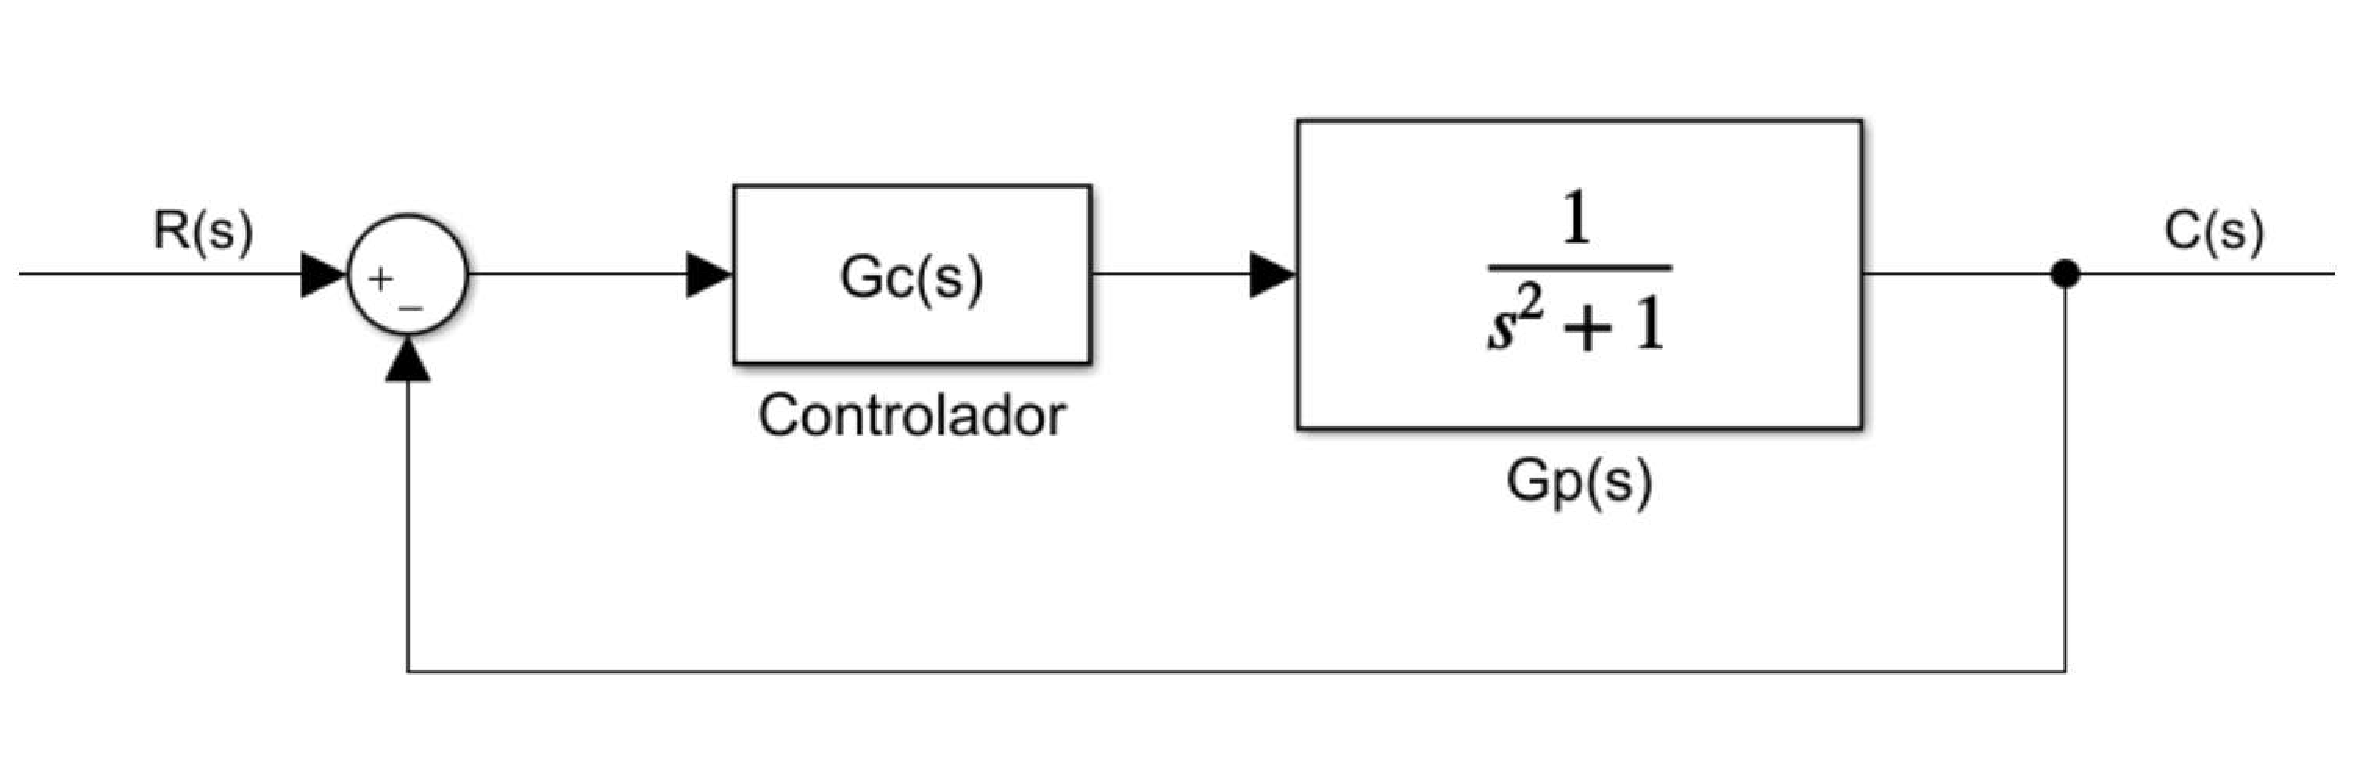
\includegraphics[width=0.8\textwidth]{Auxiliar_4_8}
  \caption{Curva característica \(v\)-\(i\) del voltaje \(v_X\) (curva azul). 
  Se intersecta la recta de carga (curva verde) con esta curva exponencial, para encontrar el punto de operación. 
  Los puntos verdes de los extremos de la recta corresponden a los puntos usados para generarla. 
  El punto verde del medio es el punto de operación del diodo si asumimos que el voltaje máximo es de \(0{,}7~\text{V}\). 
  Notemos que este punto está suficientemente cerca de la intersección real entre ambas curvas, por lo que el modelo de fuente de voltaje es una aproximación razonable.}
  \label{fig:carac-v-i}
\end{figure}
% --- Fragmento listo para pegar en tu documento ---


Luego, para el circuito de la derecha, se cumplirá que:
\begin{align*}
&\text{Cuando } v_X > 3~\text{V} \;\Rightarrow\; v_Z = -3~\text{V},\\
&\text{Cuando } v_X < 0.7~\text{V} \;\Rightarrow\; v_Z = 0.7~\text{V}.
\end{align*}

\begin{figure}[H]
  \centering
  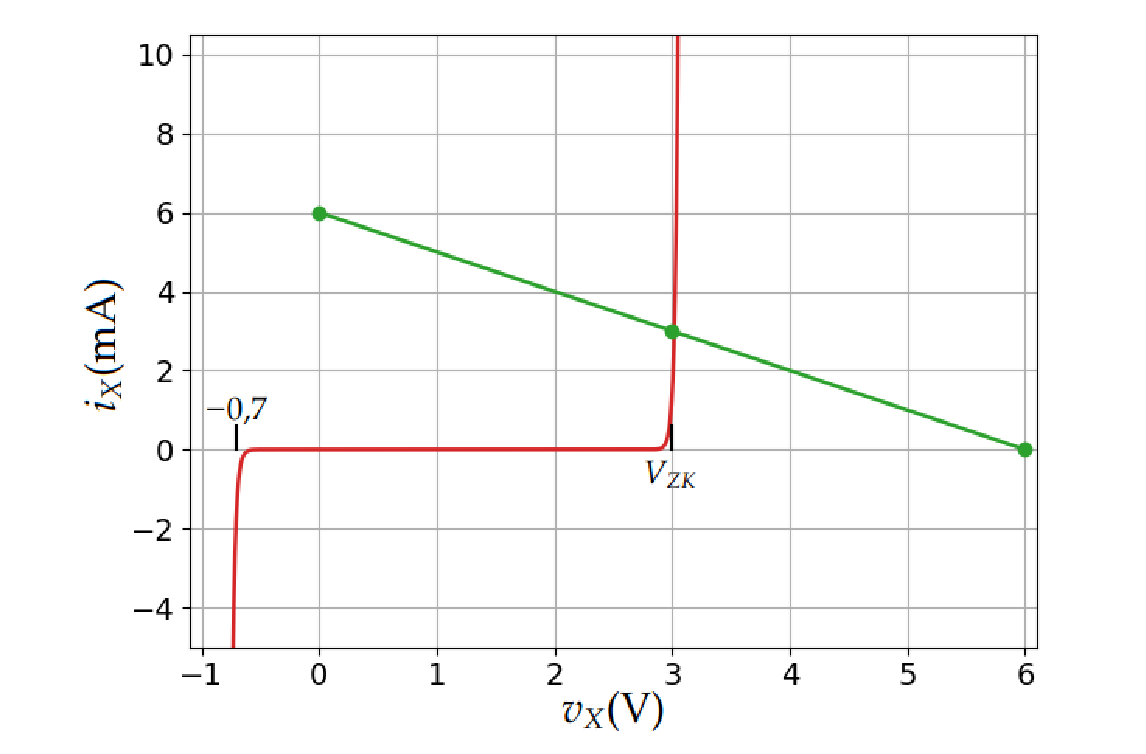
\includegraphics[width=0.8\textwidth]{Auxiliar_4_9}
  \caption{Característica $v$--$i$ del voltaje $v_X$ (recordar que el diodo Zener está invertido, por lo que la región de polarización inversa, que corresponde a voltajes negativos para el diodo Zener, en este gráfico está como voltajes positivos. Notar que la corriente también cambia de signo por la misma razón). Se intersecta la recta de carga con esta curva exponencial, para encontrar el punto de operación.}

  \label{fig:iv-diodo}
\end{figure}
Si usamos el modelo de fuente de voltaje con \(v_Z = -3~\text{V}\), tenemos que la corriente es:
\begin{align}
i_X \;=\; \frac{6 -3 }{1000} \;=\; 3~\text{mA}.
\end{align}
\end{solution}
%----------------------------
\newpage
\question Para el circuito de la figura \ref{fig:3}, bosqueje el voltaje en el diodo y la corriente en el diodo como función del tiempo. Sea explícito en los valores de las gráficas, así como en los modelos y supuestos utilizados.
\begin{figure}[H]
  \centering
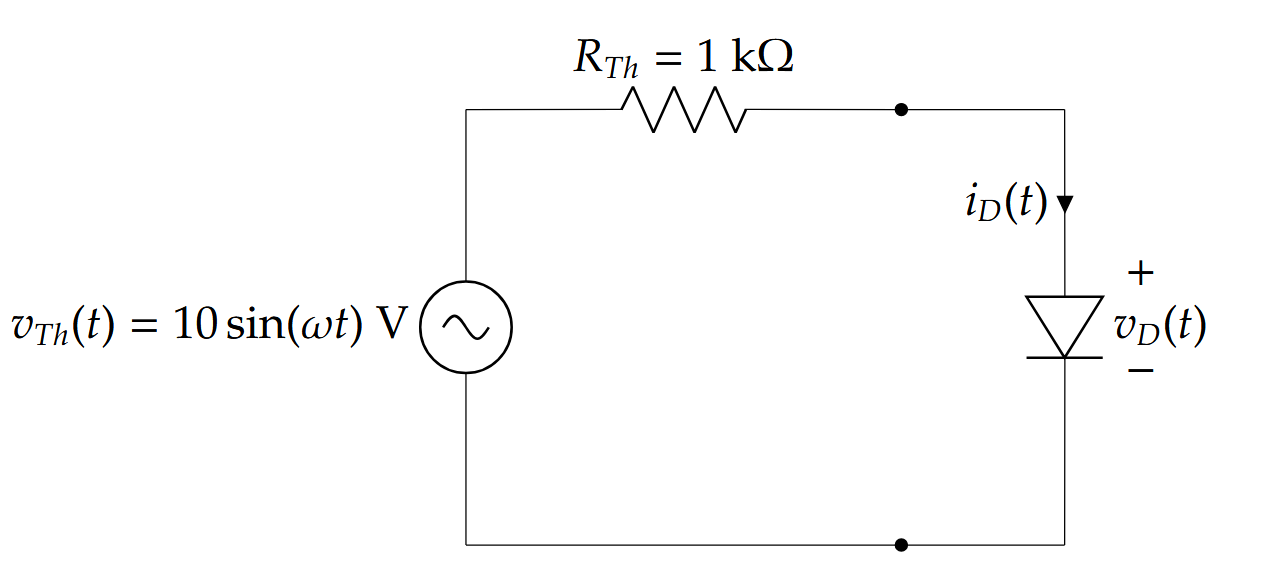
\includegraphics[width=0.7\textwidth]{Auxiliar_4_12}
  \caption{Circuito con diodo y fuente de voltaje senoidal.}
  \label{fig:3}
\end{figure}
\begin{solution}
Para poder entender cómo funciona el diodo en presencia de una fuente de voltaje senoidal, primero debemos analizar diferentes puntos, los cuales se visualizan en la tabla \ref{tab:diodo-operacion}:

\begin{table}[H]
  \centering
  \begin{tabular}{c c c c c c}
    \hline
    Punto de operación & $\omega t$ & $\sin(\omega t)$ & $v_{Th}(t)$ (V) & $v_D$ (V) & $i_D$ (mA) \\
    \hline
    3 & 0 & 0 & 0 & 0 & 0 \\
    2 & $\pi/6$ & 1/2 & 5 & 0.7 & 4.3 \\
    1 & $\pi/2$ & 1 & 10 & 0.7 & 9.3 \\
    2 & $5\pi/6$ & 1/2 & 5 & 0.7 & 4.3 \\
    3 & $\pi$ & 0 & 0 & 0 & 0 \\
    4 & $7\pi/6$ & -1/2 & -5 & -5 & $\approx -I_s$ \\
    5 & $3\pi/2$ & -1 & -10 & -10 & $\approx -I_s$ \\
    4 & $11\pi/6$ & -1/2 & -5 & -5 & $\approx -I_s$ \\
    3 & $2\pi$ & 0 & 0 & 0 & 0 \\
    \hline
  \end{tabular}
  \caption{Valores de voltaje y corriente en el diodo para distintos puntos de operación durante un ciclo senoidal.}
  \label{tab:diodo-operacion}
\end{table}
Luego, el punto de operación del diodo se ve modificado continuamente debido a la naturaleza senoidal de la fuente de voltaje; esto se observa en:
\begin{figure}[H]
    \centering
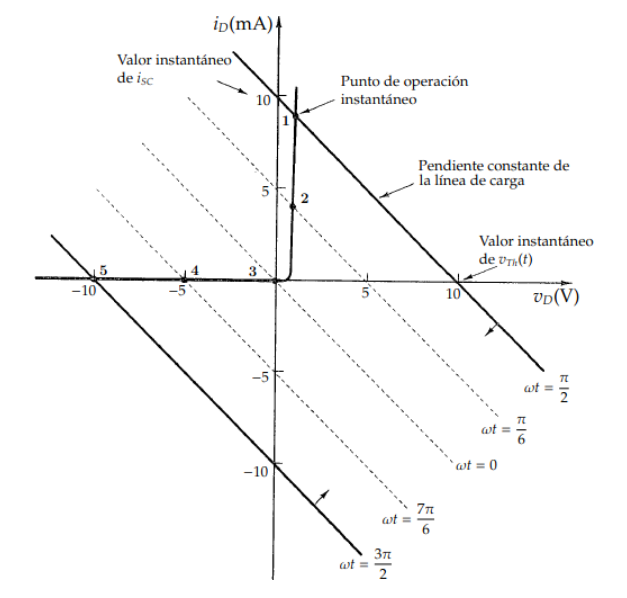
\includegraphics[width=0.7\textwidth]{Auxiliar_4_17}
    \caption{Voltaje de Thévenin $v_{Th}(t)$ como función del tiempo.}
    \label{fig:voltaje-th}
\end{figure}

\begin{figure}[H]
  \centering
  \begin{subfigure}[b]{0.48\textwidth}
    \centering
    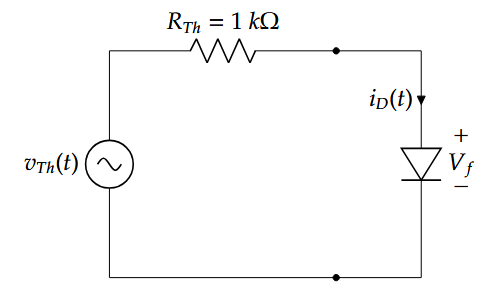
\includegraphics[width=0.9\linewidth]{Auxiliar_4_13}
    \caption{Circuito equivalente cuando el diodo no conduce ($i_D(t) = 0$).}
    \label{fig:diodo-abierto}
  \end{subfigure}\hfill
  \begin{subfigure}[b]{0.48\textwidth}
    \centering
    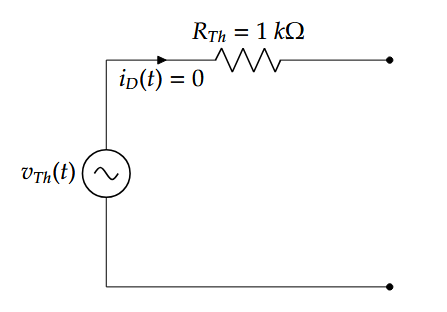
\includegraphics[width=0.9\linewidth]{Auxiliar_4_14}
    \caption{Circuito equivalente cuando el diodo conduce ($i_D(t) > 0$).}
    \label{fig:diodo-conduce}
  \end{subfigure}
  \caption{Modelos de operación del circuito con diodo: (a) abierto, (b) conduciendo.}
  \label{fig:diodo-operacion-casos}
\end{figure}
\begin{figure}[H]
    \centering
    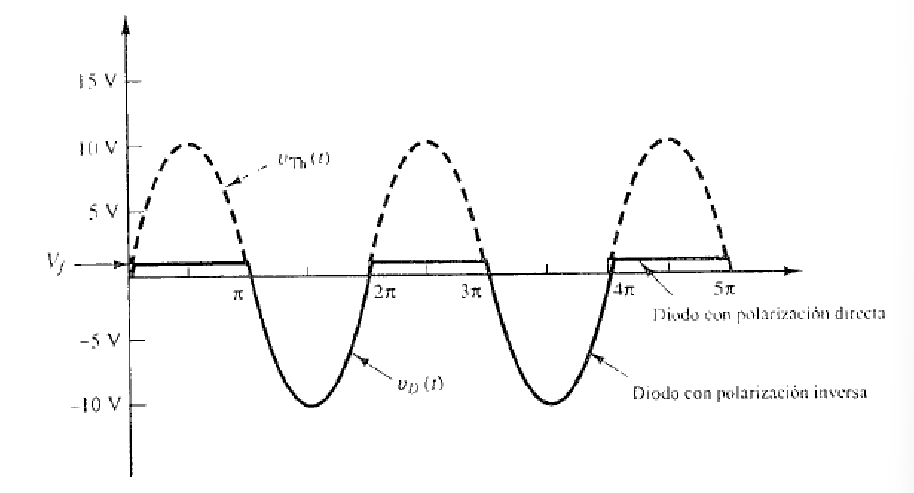
\includegraphics[width=0.55\textwidth]{Auxiliar_4_15}
  \caption{Gráfico de voltaje vs $\omega t$. Cuando el voltaje en la entrada es positivo, el voltaje medido en el diodo llega hasta un máximo de $V_f$. Cuando el voltaje en la entrada es negativo, el voltaje en la salida es igual al voltaje en la entrada por las razones descritas anteriormente.}
    \label{fig:voltaje-corriente-diodo}
\end{figure}
\begin{figure}[H]
    \centering
    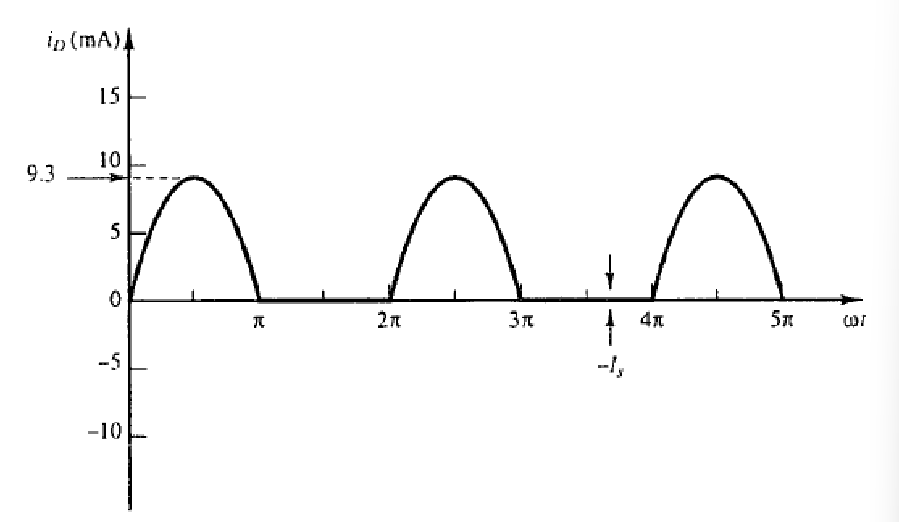
\includegraphics[width=0.55\textwidth]{Auxiliar_4_16}
  \caption{Sólo pasa corriente por el diodo cuando el voltaje es positivo (polarización directa en el diodo), porque cuando es negativo (polarización inversa en este diodo), el diodo actúa como un circuito abierto.}
    \label{fig:voltaje-corriente-diodo-detalle}
\end{figure}
\end{solution}
%----------------------------
\question Sea el esquema visto en \ref{fig:P2_17} responda lo siguiente, considerando la fuente de voltaje que ahi aparece.
\begin{enumerate}
    \item Represente (bosqueje) \(v_o\) en función del tiempo para el circuito de la Figura~\ref{fig:P2_17} (Lado izquierdo)
    con la entrada mostrada. Suponga \(V_\gamma = 0\).
    \item \textbf{[Propuesto:]} Represente (bosqueje) \(v_o\) en función del tiempo para el circuito de la
  Figura~\ref{fig:P2_17} (Lado derecho). La entrada es senoidal y está dada por
  \(v_i(t) = 10 \sin(\omega t)\,\text{V}\). Suponga \(V_\gamma = 0\).
\end{enumerate}

\begin{figure}[H]
    \centering
    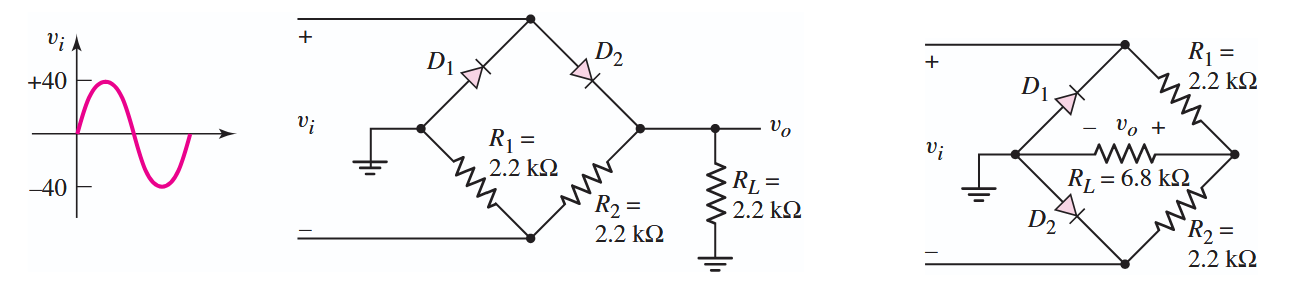
\includegraphics[width=1\textwidth]{Auxiliar_4_18}
  \caption{Esquema del circuito con diodos.}
    \label{fig:P2_17}
\end{figure}
%----------------------------
\begin{solution}
    \subsection*{Resolucion 4.1}
    Se busca el voltaje \(v_o(t)\) en función del tiempo. Para esto, se analiza el circuito en dos casos: cuando la fuente de voltaje es positiva y cuando es negativa, es decir tenemos esto:

  \begin{figure}[H]
    \centering
    \begin{subfigure}[b]{0.48\textwidth}
      \centering
    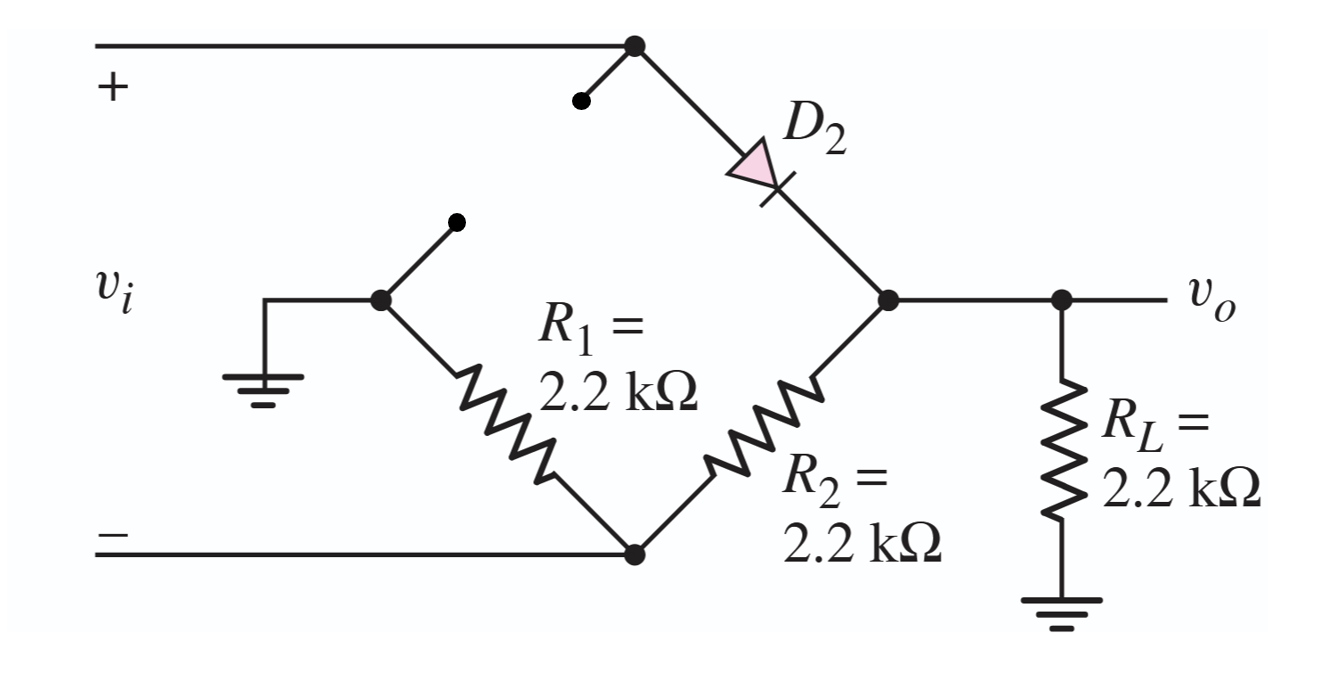
\includegraphics[width=1\linewidth]{Auxiliar_4_19}
     \caption{Caso 1: Fuente positiva. El diodo $D_1$ conduce cuando $v_i > 0$, permitiendo el paso de corriente hacia la carga.}
      \label{fig:resolucion4.1a}
    \end{subfigure}\hfill
    \begin{subfigure}[b]{0.48\textwidth}
      \centering
      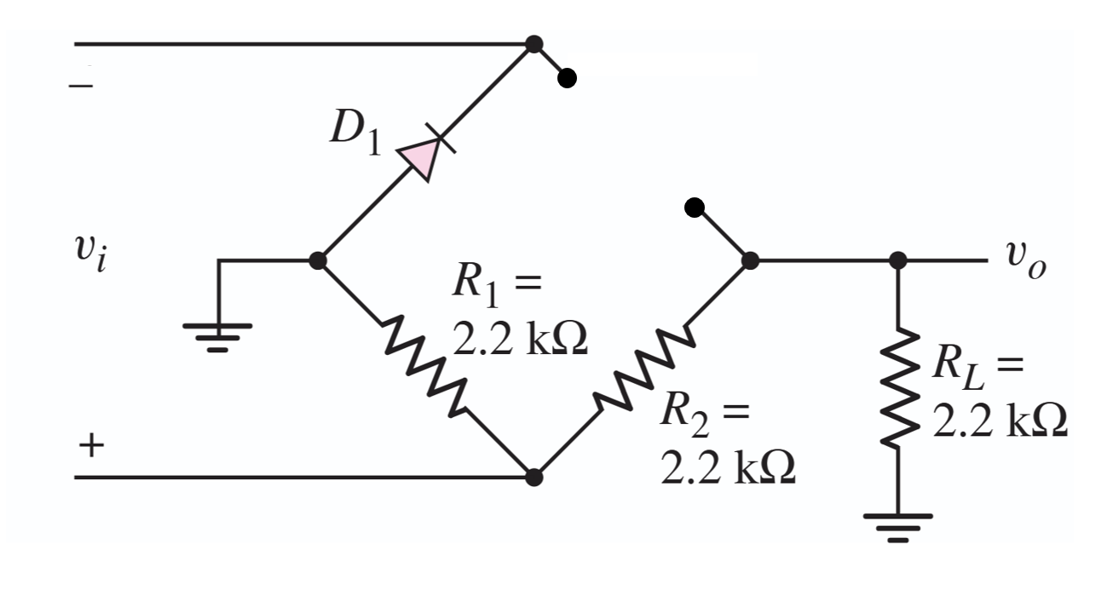
\includegraphics[width=1\linewidth]{Auxiliar_4_20}
     \caption{Caso 2: Fuente negativa. El diodo $D_2$ conduce cuando $v_i < 0$, permitiendo el paso de corriente hacia la carga en sentido opuesto.}
      \label{fig:resolucion4.1b}
    \end{subfigure}
    \caption{Análisis de los dos casos para el circuito: (a) fuente positiva y conducción por $D_1$, (b) fuente negativa y conducción por $D_2$.}
  \label{fig:resolucion4.1}
  \end{figure}
Luego tenemos que al bosquejar se obtiene lo siguiente:
\begin{figure}[H]
  \centering
  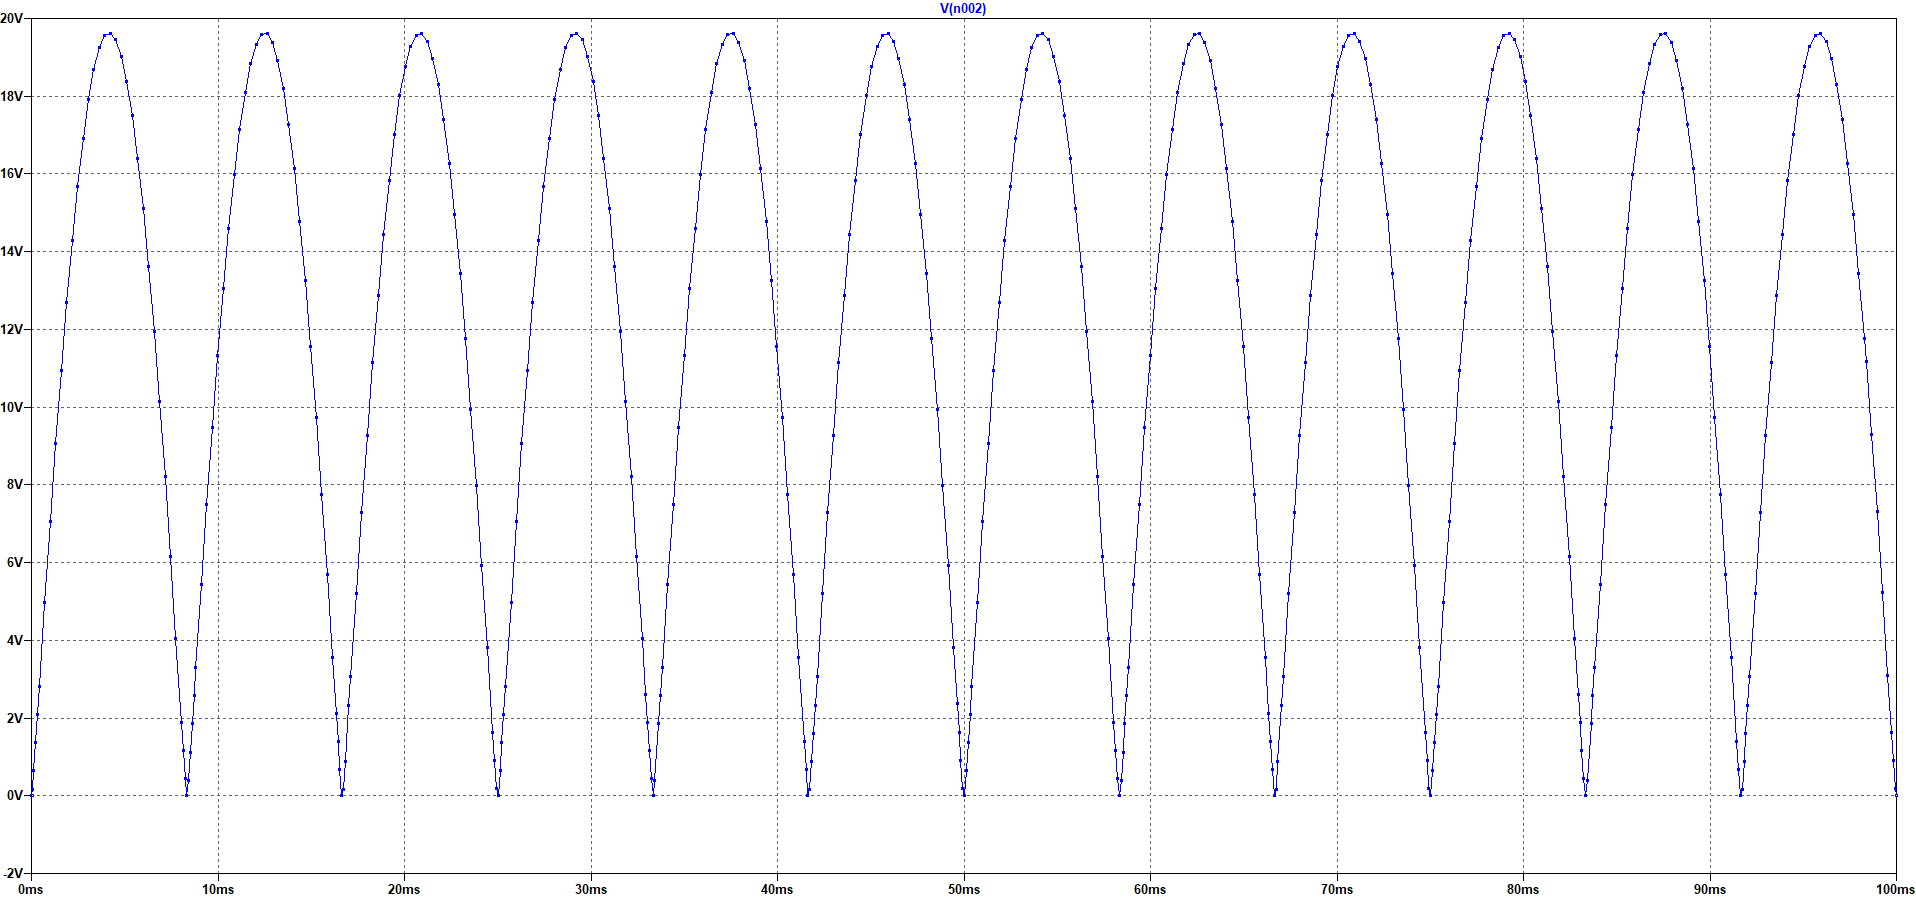
\includegraphics[width=0.7\textwidth]{Auxiliar_4_21}
  \caption{Voltaje de salida \(v_o(t)\) en función del tiempo, mostrando la forma de onda resultante del circuito con diodos.}
  \label{fig:voltaje-salida-4.1}
\end{figure}
Vemos que la amplitud del voltaje disminuye a la mitad, lo cual se puede comprobar si se realiza el circuito, es decir
\begin{figure}[H]
  \centering
  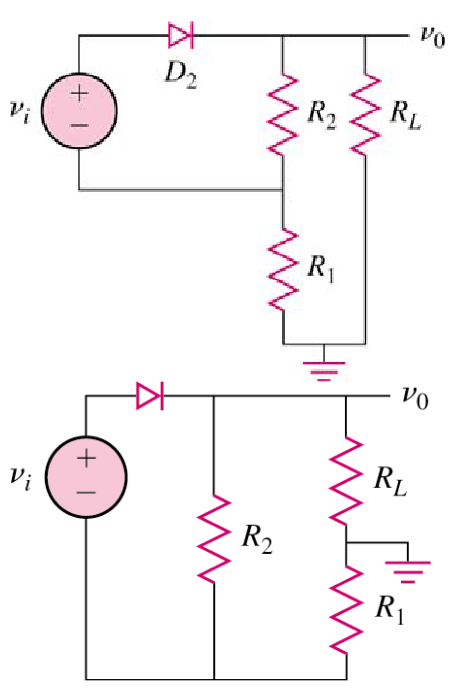
\includegraphics[width=0.4\textwidth]{Auxiliar_4_22}
  \caption{Voltaje de salida \(v_o(t)\) en función del tiempo, mostrando la forma de onda resultante del circuito con diodos.}
  \label{fig:voltaje-salida-4.1-2}
\end{figure}
Esto se debe a que el circuito actúa como un divisor de voltaje.
    \subsection*{Resolucion 4.2}
  De manera similar a lo anterior, se analiza el circuito en dos casos: cuando la fuente de voltaje es positiva y cuando es negativa, es decir, tenemos esto:

    \begin{figure}[H]
      \centering
      \begin{subfigure}[b]{0.48\textwidth}
        \centering
        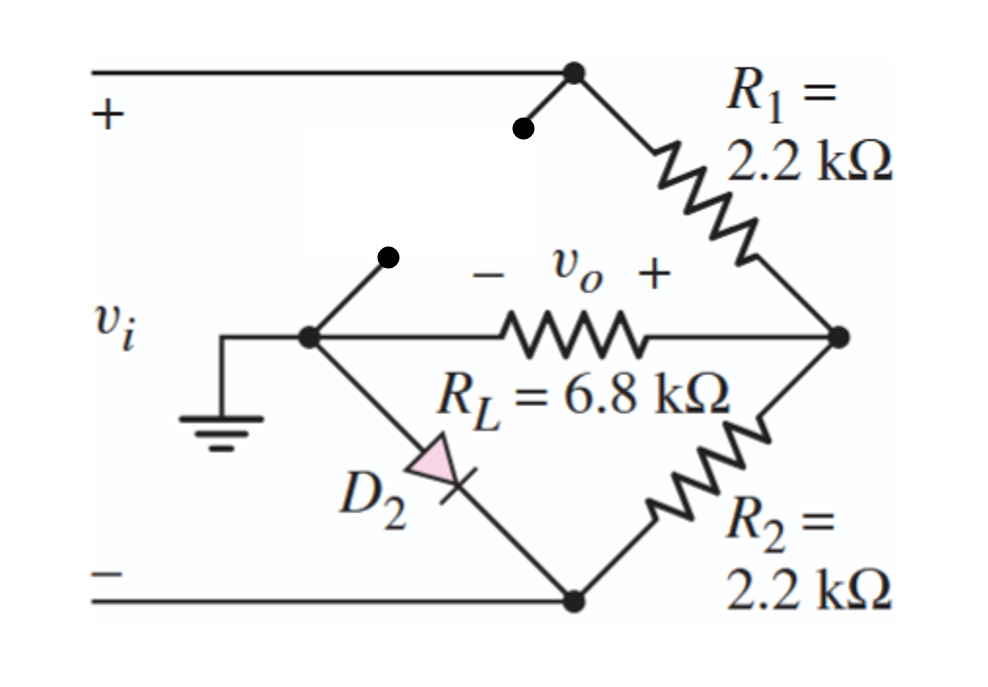
\includegraphics[width=1\linewidth]{Auxiliar_4_23}
        \caption{Caso 1: Fuente positiva. El diodo $D_2$ conduce cuando $v_i > 0$, permitiendo el paso de corriente hacia la carga.}
        \label{fig:resolucion4.2a}
      \end{subfigure}\hfill
      \begin{subfigure}[b]{0.48\textwidth}
        \centering
        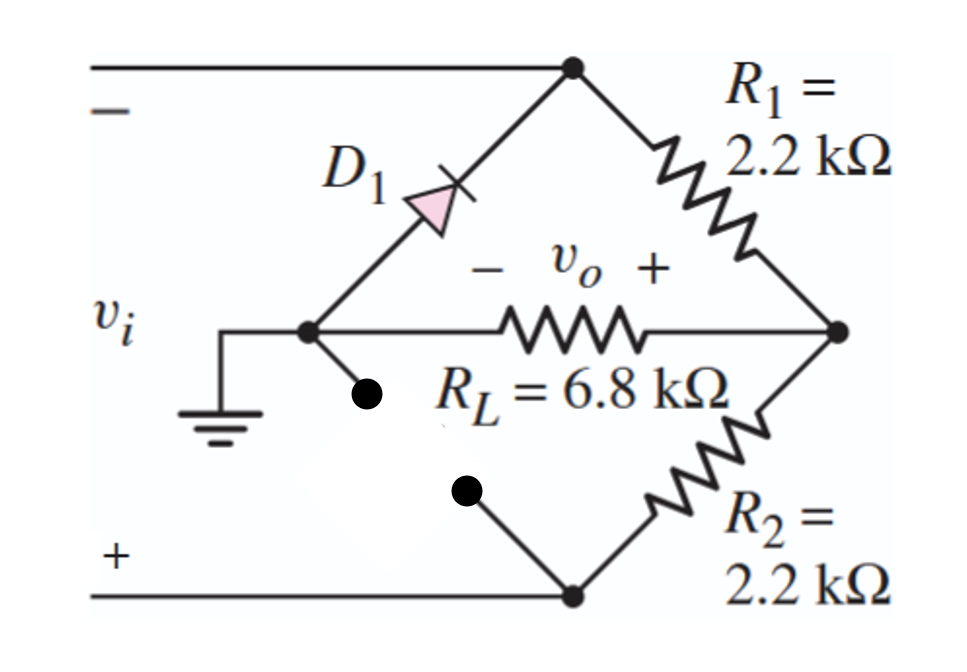
\includegraphics[width=1\linewidth]{Auxiliar_4_24}
        \caption{Caso 2: Fuente negativa. El diodo $D_1$ conduce cuando $v_i < 0$, permitiendo el paso de corriente hacia la carga en sentido opuesto.}
        \label{fig:resolucion4.2b}
      \end{subfigure}
      \caption{Análisis de los dos casos para el circuito: (a) fuente positiva y conducción por $D_2$, (b) fuente negativa y conducción por $D_1$.}
      \label{fig:resolucion4.2}
    \end{figure}
Luego tenemos que al bosquejar se obtiene lo siguiente:
\begin{figure}[H]
  \centering
  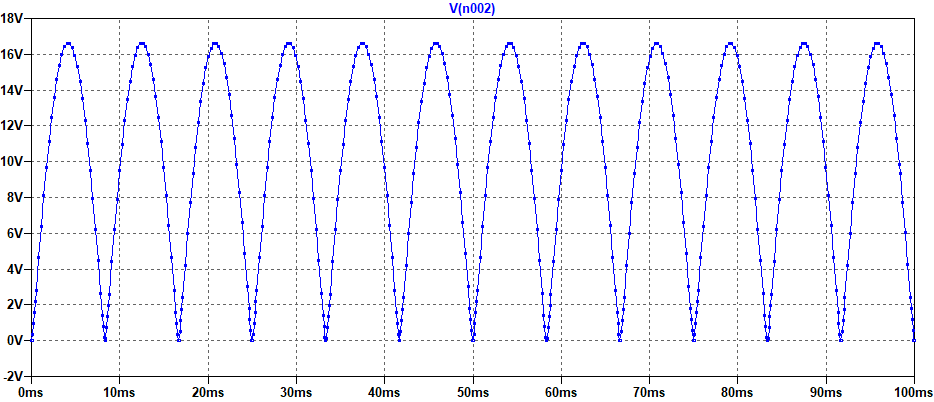
\includegraphics[width=0.7\textwidth]{Auxiliar_4_26}
  \caption{Voltaje de salida \(v_o(t)\) en función del tiempo, mostrando la forma de onda resultante del circuito con diodos.}
  \label{fig:voltaje-salida-4.2}
\end{figure}
\end{solution}
\end{questions}
\end{document}